\section{The affine-plane contraction menu}
\label{sec:geometry}

\subsection{Four directions, four complete plans}
Identify group $3x+y$ with $(x,y)\in\F_3^2$. The four maps
\[
 y,\qquad y-x,\qquad y-2x,\qquad x
\]
partition the points into their three fibers. These are the four parallel
classes of affine lines. They give the following ordered final blocks:
\begin{center}\small
\begin{tabular}{cl}
\toprule Direction & Final blocks, with the order used inside each block\\\midrule
$y$       & $(0,3,6)\mid(1,4,7)\mid(2,5,8)$\\
$y-x$     & $(0,4,8)\mid(1,5,6)\mid(2,3,7)$\\
$y-2x$    & $(0,5,7)\mid(1,3,8)\mid(2,4,6)$\\
$x$       & $(0,1,2)\mid(3,4,5)\mid(6,7,8)$\\
\bottomrule
\end{tabular}
\end{center}
Within each three-point block, first merge its last two vertices, then merge
the singleton with that pair. Finally contract the three block tables.
Thus every plan includes six internal merges and its final triangle.
Each pair of distinct points lies on exactly one affine line, and lines of
different directions meet in exactly one point. These two elementary facts
control the overlap of expensive operations across the four plans.

\begin{figure}[ht]
\centering
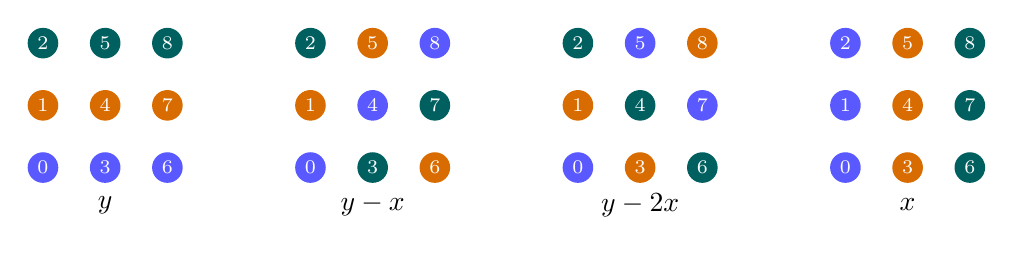
\begin{tikzpicture}[scale=.79]
\foreach \panel in {0,1,2,3}{
 \begin{scope}[xshift=4.3*\panel cm]
 \foreach \x in {0,1,2}{\foreach \y in {0,1,2}{
  \pgfmathtruncatemacro{\lab}{3*\x+\y}
  \ifnum\panel=3\pgfmathtruncatemacro{\cl}{\x}\else
  \pgfmathtruncatemacro{\cl}{mod(\y-\panel*\x+9,3)}\fi
  \ifnum\cl=0\def\clr{blue!65}\else\ifnum\cl=1\def\clr{orange!85!black}\else\def\clr{teal!75!black}\fi\fi
  \fill[\clr] (\x,\y) circle (7pt);
  \node[text=white,font=\scriptsize] at (\x,\y){\lab};
 }}
 \ifnum\panel=0\node at(1,-.6){$y$};\fi
 \ifnum\panel=1\node at(1,-.6){$y-x$};\fi
 \ifnum\panel=2\node at(1,-.6){$y-2x$};\fi
 \ifnum\panel=3\node at(1,-.6){$x$};\fi
 \end{scope}
}
\end{tikzpicture}
\caption{Each color is one final block. Coordinates and colors are interpreted
modulo three. The four plans are tested on the same exact mode-list sizes.}
\label{fig:affine}
\end{figure}

\begin{theorem}[Affine support certificate]\label{thm:affine}
For one operation support $v_j$ chosen from each of the four affine plans,
\[
 \left\|v_1+v_2+v_3+v_4\right\|_2^2\le5400.
\]
Equality is attained by every choice of four final-triangle supports.
Consequently the least-cost plan has local time and local storage coefficient
\begin{equation}
 \beta_9^2=\frac{2\cdot5400}{25\cdot4^2\cdot9^2}
   =\frac13.\label{eq:affine-beta}
\end{equation}
The construction and proof allow arbitrary internal order within each line.
\end{theorem}

\begin{proof}
There are three operation types, with tripartition sizes
$A=(1,1,7)$, $B=(1,2,6)$, and $C=(3,3,3)$. In type $A$ the two singletons
lie on the plan's affine line; in type $B$ the first two parts form that
line. For part sizes $a,b,c$, the largest squared support norm is
\[
 25(ab+ac+bc)-21\min(ab,ac,bc).
\]
The maxima are respectively $354,458,486$, so $\|v_j\|^2\le486$.
We next prove that supports from different directions satisfy $v\cdot w\le288$.

Let $S_v$ be the nonzero support and $D_v$ the discounted subset. If
\[
 c=|S_v\cap S_w|,\quad a=|D_v\cap S_w|,\quad
 b=|D_w\cap S_v|,\quad t=|D_v\cap D_w|,
\]
then
\begin{equation}
 v\cdot w=25c-15(a+b)+9t,\qquad t\le\min(a,b).\label{eq:dot-count}
\end{equation}
The expression $-15(a+b)+9\min(a,b)$ decreases with either $a$ or $b$.
The following elementary counts cover all six type pairs.

For $AA$, each support is all edges incident to two selected collinear
points. Two such pairs on transverse lines are disjoint or meet once.
Their common incident edges number at most nine: the eight edges at the
common point, and the edge between the other two selected points.
Thus the dot product is at most $225$.

For $AB$, enlarge the $B$ support to all edges incident to its entire line.
A transverse two-point set and three-point line have at most ten common
incident edges, giving $250$. For $AC$, the two selected points lie in
different lines of the other parallel class. Each has six crossing
neighbors, with their mutual edge counted twice, so $c=11$ and the bound
is $275$.

For $BB$, two transverse underlying lines meet at $x$. Their full incident
edge sets share twelve edges: eight at $x$ and four between the other two
points on each line. The omitted internal pair edge removes one common
edge unless that operation's singled vertex is $x$. Unless both singled
vertices are $x$, $c\le11$ and the dot product is at most $275$.
If both are $x$, the three possible discounts each meet the common support
in at least two edges. Hence~\eqref{eq:dot-count} gives at most
$300-15(2+2)+9\cdot2=258<275$.

For $BC$, the underlying three-point line meets each line of the other
parallel class once. Of the fifteen crossing edges incident to it, the
$B$ support omits one, so $c=14$. A $C$ discount meets the $B$ support
in at least four edges. A $B$ discount meets the $C$ support in respectively
two, four, or eight edges. Thus the dot product is at most
$350-15(4+2)+9\cdot2=278$.

For $CC$, the two internal-line edge sets are disjoint and each has nine
edges, giving $c=36-9-9=18$. Each discount has six edges crossing the other
partition. The two chosen lines from each direction make a $2$-by-$2$ grid;
its two diagonals are the common discounted edges. Thus $a=b=6,t=2$ and
\[
 v\cdot w=25\cdot18-15\cdot12+9\cdot2=288.
\]
The resulting valid upper table is
\[
\begin{array}{c|rrr}&A&B&C\\\hline
 A&225&250&275\\B&250&275&278\\C&275&278&288
\end{array}
\]
and all entries are at most $288$. Expanding the squared sum now gives
$4\cdot486+2\cdot6\cdot288=5400$.
For four final supports, every individual squared norm is $486$ and every pairwise
dot product is $288$, so equality holds. Lemma~\ref{lem:average} proves
\eqref{eq:affine-beta}.
\end{proof}

This proof establishes a bound for every feasible entropy vector, rather
than sampling random tensor dimensions. The finite checker independently
constructs all supports and verifies the norm and dot-product inequalities.
A separate exhaustive check of all $21^4=194481$ four-tuples gives the same
maximum, with exactly $3^4=81$ maximizers. Their squared norms sum to
$622974240$, an auxiliary reproducibility value.

\subsection{An exact plan selector}
For unordered edge $e=\{g,h\}$ define the positive integer
$d_e=|\mathcal I_{gh}|\,|\mathcal I_{hg}|$. For plan $j$, compute
\begin{equation}
 P_j=\max_{v\in\mathcal V_j}\prod_e d_e^{v_e}.\label{eq:selector}
\end{equation}
Its logarithm is $5F_j(g)$, so choosing the least $P_j$, with fixed-index
tie breaking, chooses the least-cost plan exactly. The number of supports
is fixed; the product bit lengths are polynomial. Empty lists are excluded
before this selector is called. No numerical optimization is executed by
the contraction algorithm.

\section{The other certified menus}
\label{sec:other-menus}

\subsection{A twelve-group certificate with a small combinatorial core}
At the second recursion level use the following four ordered plans:
\begin{center}\small
\begin{tabular}{cl}
\toprule Plan & Final blocks\\\midrule
0 &$(0,1,2,3)\mid(4,5,6,7)\mid(8,9,10,11)$\\
1 &$(9,6,4,0)\mid(1,7,10,11)\mid(5,3,2,8)$\\
2 &$(1,2,10,4)\mid(3,11,6,9)\mid(7,0,8,5)$\\
3 &$(0,5,10,11)\mid(3,8,1,6)\mid(4,9,7,2)$\\
\bottomrule
\end{tabular}
\end{center}
Within each four-point block, merge its first pair and its last pair, then
merge those pairs. The order in the table is part of the certificate.
There are thirty supports per plan, of types $A=(1,1,10)$,
$B=(2,2,8)$, and $C=(4,4,4)$.

\begin{proposition}[Twelve-group bound]\label{prop:twelve}
For these four plans the exact maximum squared sum of supports is
$Q=9864$. Therefore $\beta_{12}^2=137/400$.
\end{proposition}
\begin{proof}
The individual squared-norm maxima are $504,816,864$ for $A,B,C$.
For the six pairs of distinct plans, direct integer counts using
\eqref{eq:dot-count} give the cross-dot upper table
\[
\begin{array}{c|rrr}&A&B&C\\\hline
 A&504&500&400\\B&500&516&500\\C&400&500&540.
\end{array}
\]
This finite table can be verified from the displayed vertex sets, and the
checker reconstructs all six $30$-by-$30$ matrices. If a support tuple has
an internal operation, single it out. Its squared norm is at most $816$ and each
of its three cross dots is at most $516$. The other three squared norms are at
most $864$, with mutual dots at most $540$. Thus the squared norm of the sum is at most
\[
 816+3\cdot864+2(3\cdot516+3\cdot540)=9744.
\]
It remains to examine the three final supports in each plan. Index them
by their discounted class, in order $(0,1),(0,2),(1,2)$. Their pairwise
dot product is $540$ when $x_j=p_{ij}(x_i)$ and $522$ otherwise, where
\[
\begin{array}{c|rrrrrr}
 ij&01&02&03&12&13&23\\\hline
 (p_{ij}(0),p_{ij}(1),p_{ij}(2))
 &(1,2,0)&(1,0,2)&(2,0,1)&(0,2,1)&(1,2,0)&(2,1,0).
\end{array}
\]
These six tiny matrices are also checked directly. Triangles $012,023,123$
are inconsistent: for every $x$, $p_{jk}(p_{ij}(x))\ne p_{ik}(x)$.
Only triangle $013$ is consistent. Five edges of $K_4$ contain two
triangles, so five preferred relations cannot hold at once. At most four
pairs have dot $540$, and four are attained at $(x_0,x_1,x_2,x_3)=(0,1,0,2)$.
Consequently
\[
 Q=4\cdot864+2(6\cdot522+4\cdot18)=9864>9744.
\]
Finally $2Q/(25\cdot4^2\cdot12^2)=137/400$.
\end{proof}
The certificate was suggested by a finite search. Its validity depends only
on the four displayed plans and the exact checks, not on the search or its
floating-point heuristic. Independent enumeration of all $30^4=810000$
tuples gives nine maximizers and squared-norm sum $3501532800$.
No global optimality over other menus is asserted.

\subsection{Puncturing the affine plane and ending the recursion}
Delete point $8$ from every affine block to obtain the eight-group menu.
Delete points $7,8$ for the seven-group menu. Keep the surviving order and
use the same balanced split rule. No block is empty. Direct exact support
certificates give
\begin{center}
\begin{tabular}{rrrrrl}
\toprule $r$ & Plans & Supports/plan & Tuples & $Q$ & $\beta_r^2$\\\midrule
9 &4&21&194481&5400&$1/3$\\
12&4&30&810000&9864&$137/400$\\
8 &4&18&104976&4464&$279/800$\\
7 &4&15&50625&3564&$891/2450$\\
4 &1&6&6&104&$13/25$\\
\bottomrule
\end{tabular}
\end{center}
The four-group plan is simply $(0,1)\mid(2)\mid(3)$. Its two operations
both have tripartition sizes $(2,1,1)$, up to ordering, and the largest
squared support norm is $104$. The punctured certificates are finite
integer exhaustions, not extrapolations of the nine-point geometry.
The independently reconstructed sums for $r=8,7$ are respectively
$289547136$ and $118219500$.

The compact certificate theorem improves the menu coefficients within the
current mode-entropy model. It does not assert that every algebraic entropy
vector is realized by a SAT instance, that the chosen tree is globally
optimal, or that tensor contraction requires explicit tables in every
possible representation.
